
\begin{frame}
    \frametitle{Что такое ГИС?}
    \begin{description}
        \item[Геоинформационная система; ГИС:] Информационная система,
        оперирующая пространственными данными [ГОСТ Р 52438-2005];

        \item[информационная система:] Система, предназначенная для хранения,
        обработки, поиска, распространения, передачи и
        представления информации [ГОСТ 7.0-99];

        \item[информационная система:] совокупность содержащейся в базах
        данных информации и обеспечивающих ее обработку информационных т
        ехнологий и технических средств [N 149-ФЗ].

    \end{description}

    Геоинформационная система (ГИС) ---
    система сбора, хранения, анализа и графической визуализации
    пространственных (географических) данных и связанной с ними
    информацией о необходимых объектах.

\end{frame}

\begin{frame}
    \frametitle{Что такое ГИС?}
    \begin{figure}[!ht]
        \begin{center}
            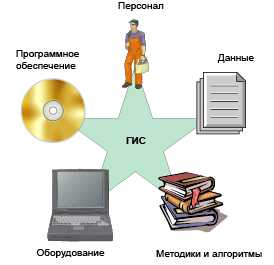
\includegraphics[width=0.4\columnwidth]{./introduction/img/what-is-gis.png}
        \end{center}
    \end{figure}
    Совокупность программно-аппаратных средств, обученного персонала,
    способных создавать, хранить, показывать и анализировать данные о
    расположении и свойствах объектов в пространстве.
\end{frame}
\note{
Сказать, что все части важны. Обратить
внимание, что тут нет ни слова про
карту, потому что ГИС --- это не карта, пусть даже электронная.
ГИС --- это гораздо больше.

Перейти к тому, что ниже мы будем рассматривать не все
компоненты, а только то, что нас интересует больше всего:
\begin{itemize}
    \item Данные;
    \item Методики;
    \item ПО;
\end{itemize}
}
